\documentclass[11pt, a5paper, parskip=half-, DIV=12]{scrartcl}

\usepackage{../endeavour}
\usepackage{../endeavour_book}

\version{0.1}

\begin{document}
% Colour Cover
\thispagestyle{plain}
\AddToShipoutPictureBG{
\begin{tikzpicture}[remember picture, overlay]
	\node () at (current page.center) {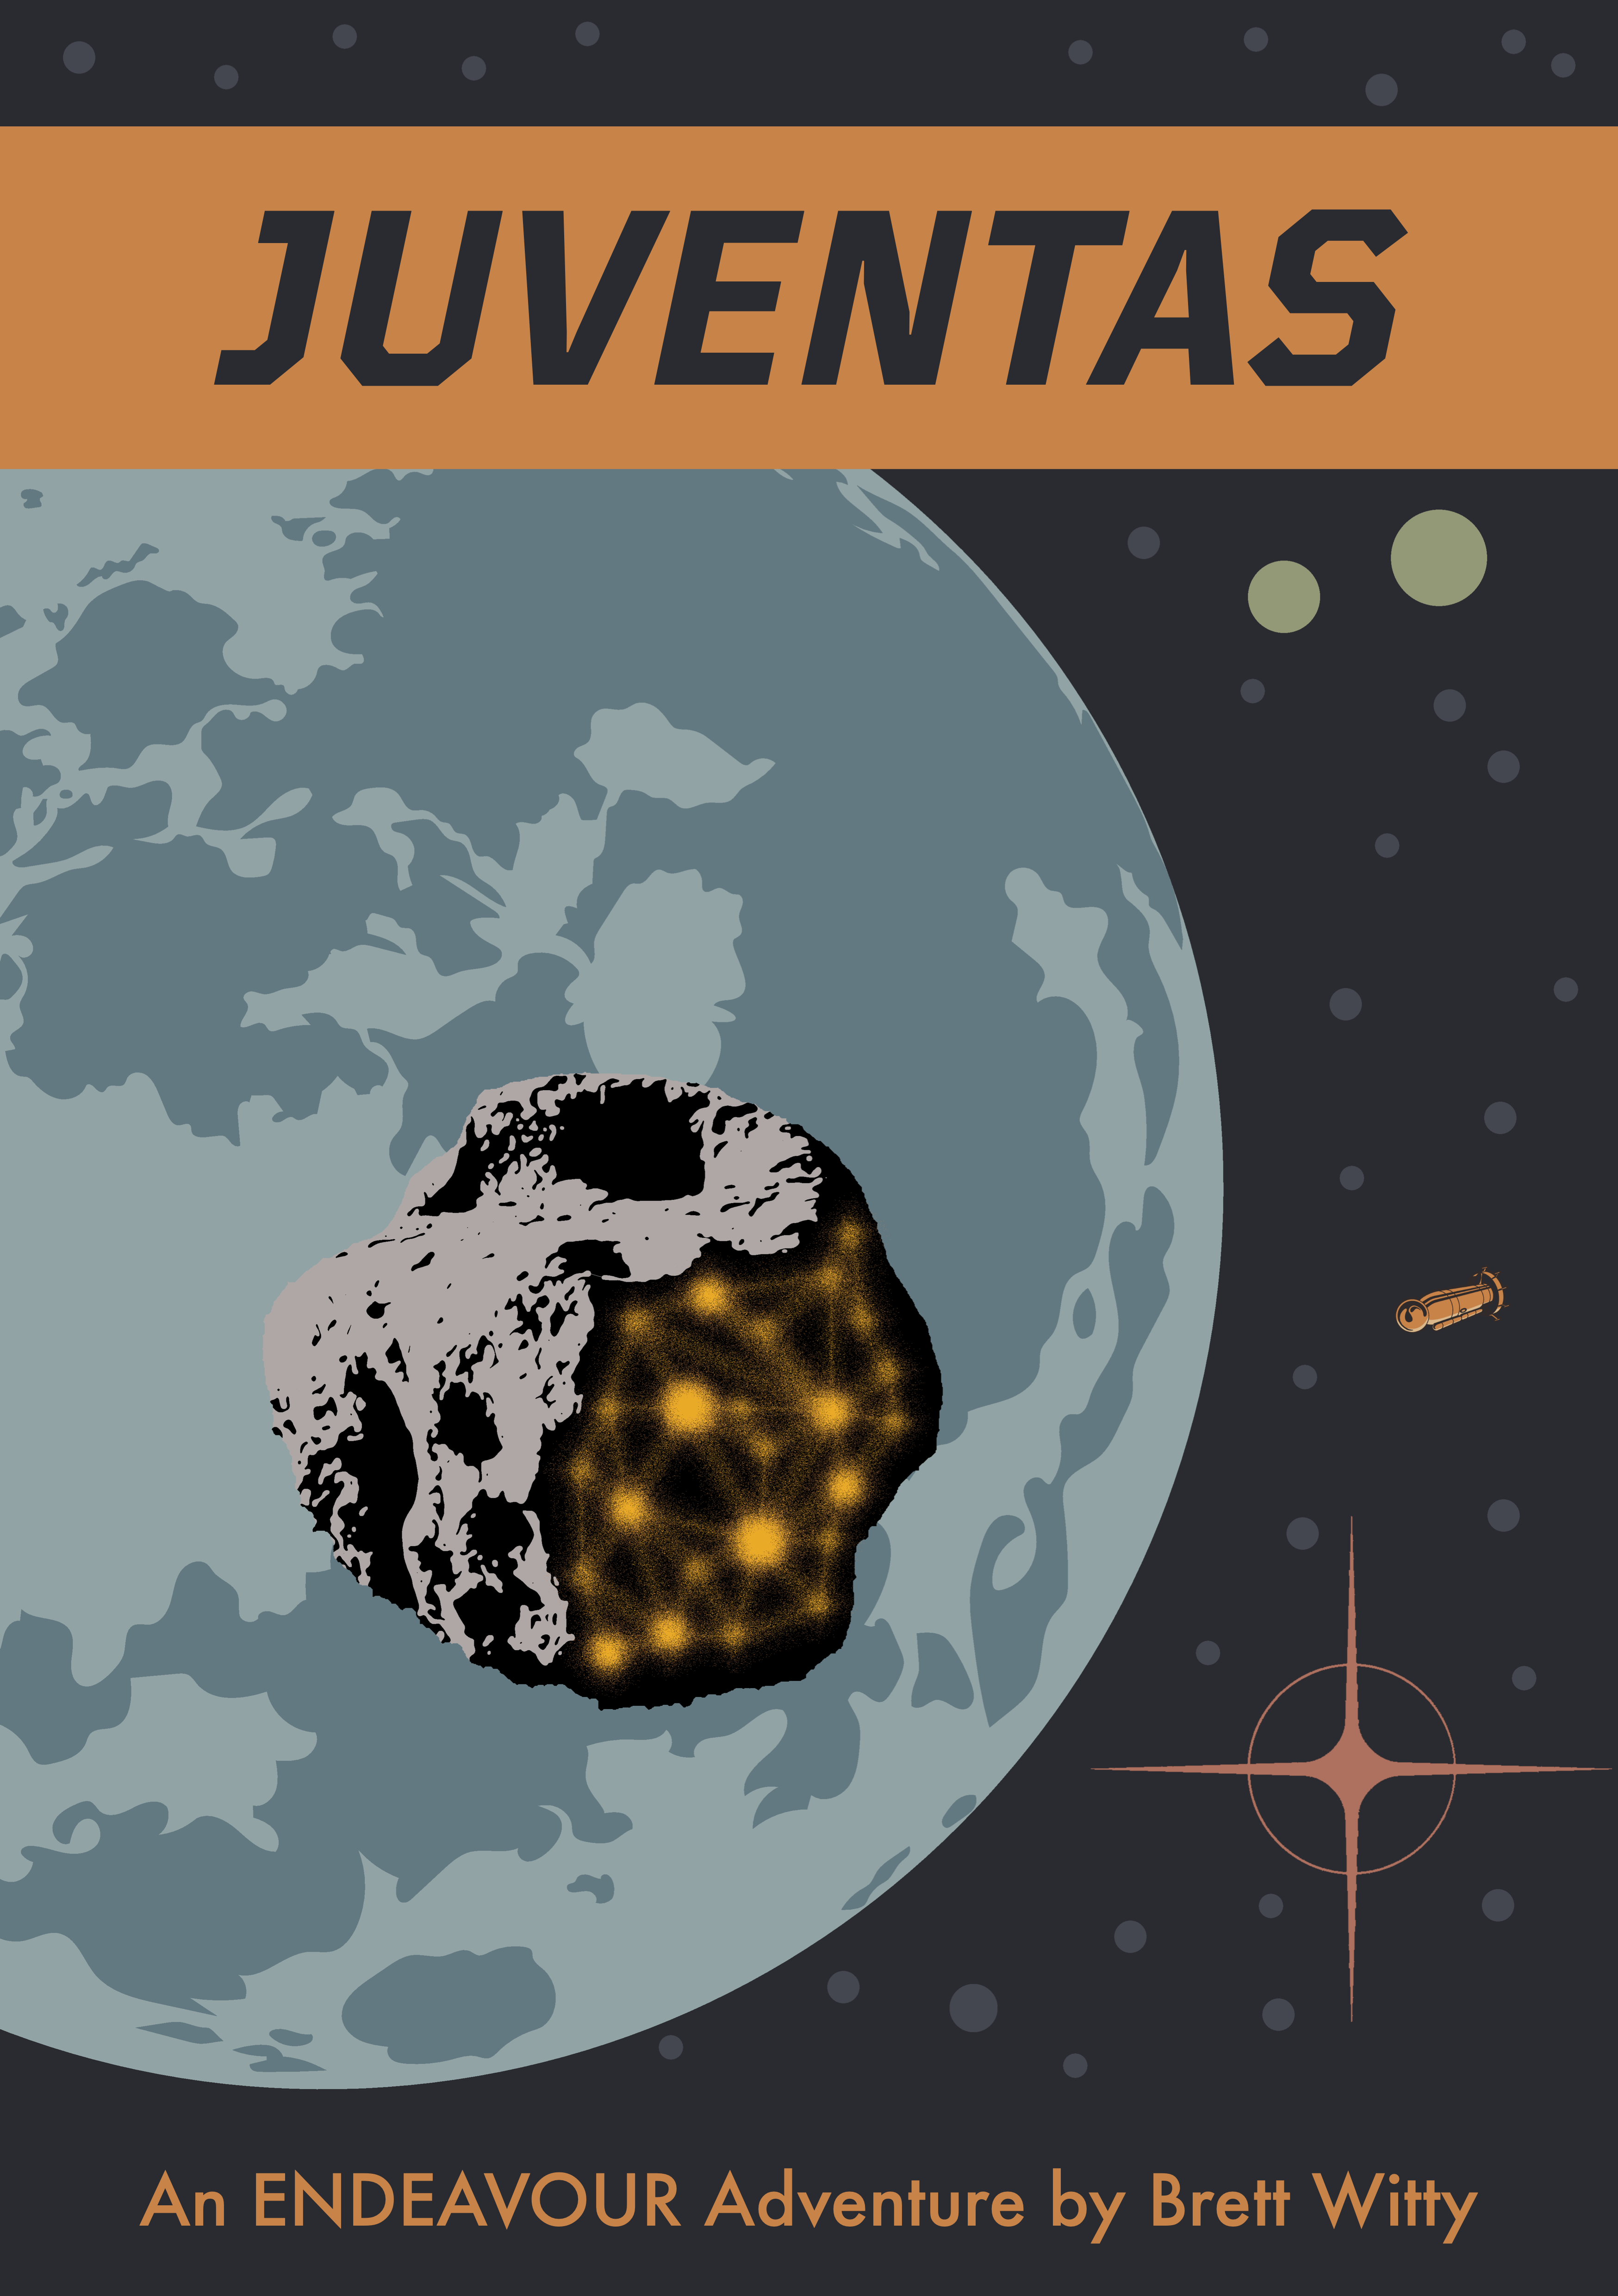
\includegraphics[width=\pagewidth, height=\pageheight]{Images/juventas_cover.png}};
\end{tikzpicture}
}
{
\colorlet{headfootcolor}{LCARS_ORANGE}
\phantom{a}

\newpage
}

\ClearShipoutPicture
\AddToShipoutPictureBG{
	\begin{tikzpicture}[remember picture, overlay]
	\pic () at (current page.center) {starfield};
		\node[endeavour_box, minimum width=12.6cm, minimum height=18.8 cm] at (current page.center) {};
	\end{tikzpicture}
}

\setcounter{page}{1}
\setmainfont{TeX Gyre Schola}
\normalsize
\raggedright

\section*{Juventas}
\textit{\textbf{Captain's Log:} Whilst returning from deep space, our engineers have identified rare, systemic damage to the Endeavour’s energy calibration matrix. ICF Command have identified Juventas, a moonlet orbiting Edda II, as a source of expertise and equipment to rectify this problem.}

\textit{ Juventas, however, is outside of Interstellar Confederation space and is well-known for its anarchic community of engineers, poets, makers, writers, and tinkers. As official representatives of the ICF, we are unlikely to be welcome. Nevertheless, we must find someone willing to help us here.}

\subsection*{Arrival}
You dock with the hollowed-out moonlet which is ablaze in clashing neon
lighting and densely interconnected habitation modules. Shortly after you arrive, the power drops out temporarily before a secondary backup brings most systems back online. The Endeavour desperately needs repairs.

As you disembark, two hovering robots approach and demand to know who you are and why you are here. They accept your answers and disappear into a tunnel nearby. The locals take little notice of you and continue on with their own business in what feels like an endless marketplace and artists' commune.

\subsubsection*{At Loose Ends}
\begin{itemize}
	\item \textit{Will you try to convince the locals to help you find someone who can help you repair the energy calibration matrix?} \\ \textbf{Leadership \& Negotiation} vs. \textbf{The Commune}.
	\item \textit{Or will you try to navigate the marketplace on your own?} \textbf{Operations \& Engineering} vs. \textbf{Matrix Lacers}.
\end{itemize}
The atmosphere here is quite tense and you see several fights break out while you explore the labyrinthine space.
\newpage

\subsection*{Trials}
\subsubsection*{Too Many Troys}
At Matrix Lacers, a young technician named Lacer Troy is threatening to kill his coworkers with a grenade. He claims that they are clones and that his real coworkers are missing. \textit{Can you convince Lacer Troy to surrender peacefully and release his hostages safely?} \textbf{Leadership \& Negotiation} vs. \textbf{Lacer Troy}. This is a \textit{Dangerous} and \textit{Fraught} challenge.

\subsubsection*{Distinguishing Features}
A young man approaches you . \textit{Ask a leading question that suggests a possible challenge.} \textbf{Science \& Medicine} vs. \textbf{Piker Savat}.

\subsubsection*{Infiltration Attempt}
A set of clones is discovered trying to access the Endeavour. Drones like the ones that met the landing party observe the attempt. \textit{Can you capture one of the drones?} \textbf{Strategy \& Tactics} vs. \textbf{Piker Savat}.

\subsection*{Crisis}

\begin{itemize}
	\item \textit{Will you \ldots?} \textbf{Threats:} Two or three threats.
	\item \textit{Or will you \ldots?} \textbf{Threats:} Two or three threats.
\end{itemize}

\newpage

\subsection*{Characters}
\begin{description}
	\item[Piker Savat (d10):] Innovative (d10), Cunning (d8), Arrogant (d8), Charming (d8), Amoral (d6 \textit{Sensitive}).
	\item[Zonos (d8):] Head Lacer (d8), Clever (d8), Greedy (d8).%, Missing Hand (d6).
	\item[Lacer Troy (d8):] Lacer (d8), Paranoid (d6), Loyal (d6).
	\item[Clone (d?):] \textbf{\textsc{Doppelg\"anger}} (Clones have the same skills and memories as the person from which they were copied).\\ \textbf{\textsc{Unsettling}} (Challenges vs. one's own clone are \textit{Fraught}).
\end{description}

\subsection*{Places}
\begin{description}
	\item[Edda II:] A dangerous planet whipped by strong winds and planet-wide blue copper dust storms.
	\item[Matrix Lacers:] A pioneering workshop in energy matrix engineering. One of the few places outside the ICF and private laboratories to research this technology.
	\item[Savat's Factory:] A hidden high-tech laboratory where Piker Savat has revolutionized rapid cloning technology.
\end{description}

\subsection*{Mysteries}
\begin{description}
	\item[Juventas is home to many skilled artisans.] \phantom{} \\ Because there is no government on Juventas, it is a haven for those whose interests might be considered exotic or illegal elsewhere.  \textit{ How do they survive out here? What attracted the first denizens of Juventas to the moonlet?}
	\item[Piker Savant's clones are imperfect.] \phantom{} \\ Outwardly, the clones are identical to the person from which they were copied. Inwardly, they inevitably differ in subtle ways. \textit{What are the potential applications of this technology? How can you tell if a person is a clone? }
\end{description}

\newpage

\section*{Acknowlegements}
Much of the look and feel of \ENDEAVOUR{} is derived from its art, all of which was created by \textbf{svekloid}. This art was assembled from multiple collections available online at \href{http://shutterstock.com}{shutterstock.com} and then modified by Michael Purcell.  

\subsection*{Playtesters} \label{subsection:playtesters}
The following people helped to create \ENDEAVOUR{} by playing early versions of the game and providing invaluable feedback.\vspace{-1.75ex}
\begin{multicols}{2}
\begin{itemize}[noitemsep]
  \item Keydan Bruce
  \item Dannielle Harden
  \item Andrew Hellyer
%  \item Sarah Hewat
%  \item Scott Joblin
%  \item Sen-Foong Lim
  \item David McKenzie
%  \item Holly Moore
  \item Paul Murray
%  \item David Purcell
%  \item Heidi Purcell
  \item Kira Purcell
  \item Luke Purcell
  \item Meagan Purcell
%  \item Steve Purcell
%  \item Jason Stark
  \item Jo Stephenson
%  \item Pieter Vismans
  \item Brett Witty
  \item Bevis Worcester
  \item Evan Worcester
\end{itemize}
\end{multicols}

\subsection*{Design Tools} \label{subsection:design-tools}
The following tools were used to create this document:
\begin{description}[font=\normalfont\textbullet\space, noitemsep, topsep=-1ex]
	\item[LuaLaTeX:] Typesetting and layout.
	\item[TikZ:] Diagrams and art.
\end{description}
\vspace{1ex}
The fonts used are {\setmainfont{TT Mussels-BoldItalic} TT~Mussels~Bold~Italic},  \textsf{Futura}, and TeX~Gyre~Schola (cf. Century Schoolbook).

\vfill

\begin{tabular}{@{}m{7.775cm}@{\hspace*{0.375cm}}>{\centering\arraybackslash}m{2.6cm}@{}}
\textbf{Contact:} \href{mailto:endeavour.ttrpg@gmail.com}{endeavour.ttrpg@gmail.com}\newline \phantom{This is a test, only a test.} \newline \footnotesize{For use with the \textsc{Paragon} system, ©2020\newline \textbf{John Harper \& Sean Nittner}. \href{http://agon-rpg.com}{AGON-RPG.com}} & \includegraphics[scale=0.175]{Images/paragon_logo_mark.png} \\[5ex]
\footnotesize{This work is licensed under a Creative Commons \newline ``Attribution-ShareAlike 4.0 International'' license.} & \Huge{\doclicenseIcon}
\end{tabular}

\newpage

\thispagestyle{empty}

\tikzset{starfield/.pic={
	\node () at (current page.center) {
\includegraphics[width=\pagewidth, height=\pageheight]{Images/starfield.png}};
}}

\ClearShipoutPicture
\AddToShipoutPictureBG{
	\begin{tikzpicture}[remember picture, overlay]
	\pic () at (current page.center) {starfield};
	\end{tikzpicture}
}

\phantom{a}

\end{document}